%%%%%%%%%%%%%%%%%%%%%%%%%%%%%%%%%%%%%%%%%%%%%%%%%%%%%%%%%%%%%%%%%%
\begin{appendices}
%%%%%%%%%%%%%%%%%%%%%%%%%%%%%%%%%%%%%%%%%%%%%%%%%%%%%%%%%%%%%%%%%%
\section{Mesh sensitivity of the wave-flume case}
\label{app:flexveg_mesh}
%%%%%%%%%%%%%%%%%%%%%%%%%%%%%%%%%%%%%%%%%%%%%%%%%%%%%%%%%%%%%%%%%%

\noindent
The wave-flume case carries two resolution requirements at once, because the mesh has to propagate the incident wave without distorting it and it also has to resolve the Gaussian kernel through which the stem acts on the fluid. This appendix examines both by repeating the largest-deflection condition H110T20, at its production coefficient $C_{dn} = 2.4$, on three successively refined meshes. Everything outside the mesh is held fixed, namely the kernel width at $\varepsilon = 0.015~\mathrm{m}$, the drag coefficients, the sampling offset, the force relaxation, the wave theory and its ramp, the discretisation schemes, the solver tolerances, and the Courant limit. Table~\ref{tab:flexveg_mesh} lists the three meshes. The middle one is the production mesh of Section~\ref{sec:flexveg_setup}, on which every result reported in that section is computed, and the coarse and fine meshes are obtained from it by dividing and multiplying the cell count in each direction by $\sqrt{2}$. Each level therefore carries about $2.8$ times the cells of the one below, the three spanning a factor of eight overall, and the vertical resolution of the largest wave rises from $19$ to $38$ cells per wave height. Because $\varepsilon$ is a physical width and is held fixed, the ratio $\varepsilon/\Delta x$ rises with refinement from $1.77$ to $3.54$, so the study varies the kernel-to-cell ratio at the same time as the mesh.

\noindent
Each case contributes its last three complete wave periods, at $26$ to $32~\mathrm{s}$ on the coarse mesh, $24$ to $30~\mathrm{s}$ on the baseline, and $18$ to $24~\mathrm{s}$ on the fine mesh, the last because the fine run reached $t = 25.6~\mathrm{s}$ within its wall-clock allocation. Every window starts at an integer multiple of the wave period and the paddle forcing is exactly periodic, so the three windows are phase-locked and overlay directly. Peaks and ranges are read after band-limited interpolation of each whole-period window, because the output interval of $0.1~\mathrm{s}$ gives only twenty samples per period and places up to $1.2\%$ of sampling bias on a raw extreme, which is the same order as the mesh differences being measured.

\begin{table}[!ht]
\centering
\small
\caption{The three meshes of the wave-flume sensitivity study, run at condition H110T20 with $C_{dn} = 2.4$ and $\varepsilon = 0.015~\mathrm{m}$ held fixed. The baseline is the production mesh of Section~\ref{sec:flexveg_setup} and the other two are that mesh scaled by $\sqrt{2}$ in each direction. Cell counts are for the whole flume and the spacings are those over the plateau. $H/\Delta z$ is the number of cells per wave height and $\varepsilon/\Delta x$ the kernel width in streamwise cells. The last four columns are the base-force range $\Delta F$, the tip oscillation range $\Delta x_s$, the crest elevation $\eta_c$ at the stem, and the mean water level $\bar{\eta}$ at the stem, each taken over the last three complete wave periods. Both elevations are referenced to the still water level, whereas Section~\ref{sec:flexveg_results_wave} reports elevations about the local mean, so the two differ by $\bar{\eta}$.}
\label{tab:flexveg_mesh}
\footnotesize
\setlength{\tabcolsep}{2.5pt}
\renewcommand{\arraystretch}{1.15}
\begin{tabular}{l c c c c c c c c}
\toprule
Mesh & Cells & $\Delta x \times \Delta y \times \Delta z$ (mm) & $H/\Delta z$ & $\varepsilon/\Delta x$ & $\Delta F$ (mN) & $\Delta x_s$ (mm) & $\eta_c$ (mm) & $\bar{\eta}$ (mm) \\
\midrule
Coarse   & $4.8\times10^{6}$  & $8.5 \times 56.6 \times 5.8$ & $19$ & $1.77$ & $173.2$ & $99.6$  & $65.9$ & $+1.0$ \\
Baseline (prod.) & $1.35\times10^{7}$ & $6.0 \times 40.0 \times 4.1$ & $27$ & $2.50$ & $170.3$ & $97.7$  & $74.4$ & $+9.1$ \\
Fine     & $3.8\times10^{7}$  & $4.2 \times 28.3 \times 2.9$ & $38$ & $3.54$ & $173.6$ & $100.4$ & $73.3$ & $+6.8$ \\
\bottomrule
\end{tabular}
\end{table}

\noindent
The load and the response are converged from the baseline mesh upward. The base-force range is $173.2$, $170.3$ and $173.6~\mathrm{mN}$ on the three meshes, so the baseline sits $1.9\%$ below the fine mesh, and the tip oscillation range is $99.6$, $97.7$ and $100.4~\mathrm{mm}$, a baseline deviation of $2.7\%$. The range of the upstream-sampled velocity that drives the drag agrees to within $2\%$ on all three meshes. One qualification belongs with those numbers. The per-period tip range is constant to $\pm0.1\%$ on the coarse and the baseline meshes, but the fine run is still drifting downward by about $0.4\%$ per period, so its own range is converged only to roughly $\pm1\%$, which is the same order as the deviations quoted. That drift runs toward the baseline value, so a fully settled fine run would improve the agreement rather than worsen it.

\noindent
Figure~\ref{fig:flexveg_mesh_force} shows that the visible difference on the coarse mesh is phase rather than magnitude. In the difference panel the coarse curve departs from the fine one by up to $13~\mathrm{mN}$ on a range of $173~\mathrm{mN}$, which reads as a substantial load error, but its range is within $0.24\%$ of the fine mesh and it is the baseline that is the outlier in magnitude. The whole of the visible difference is a first-harmonic phase lag of $8.85^{\circ}$, which is $2.5\%$ of a period and accounts for $2 \times 81.9~\mathrm{mN} \times \sin(8.85^{\circ}/2) = 12.6~\mathrm{mN}$. The same lag of $8.7$ to $9.6^{\circ}$ appears in the surface elevation, in the sampled velocity, in the base force, and in the tip displacement, and the lags between those four quantities are mesh-independent to under $1^{\circ}$. The coarse mesh therefore propagates the wave slightly too slowly, and the coupling introduces no mesh-dependent lag of its own.

\begin{figure}[!ht]
\centering
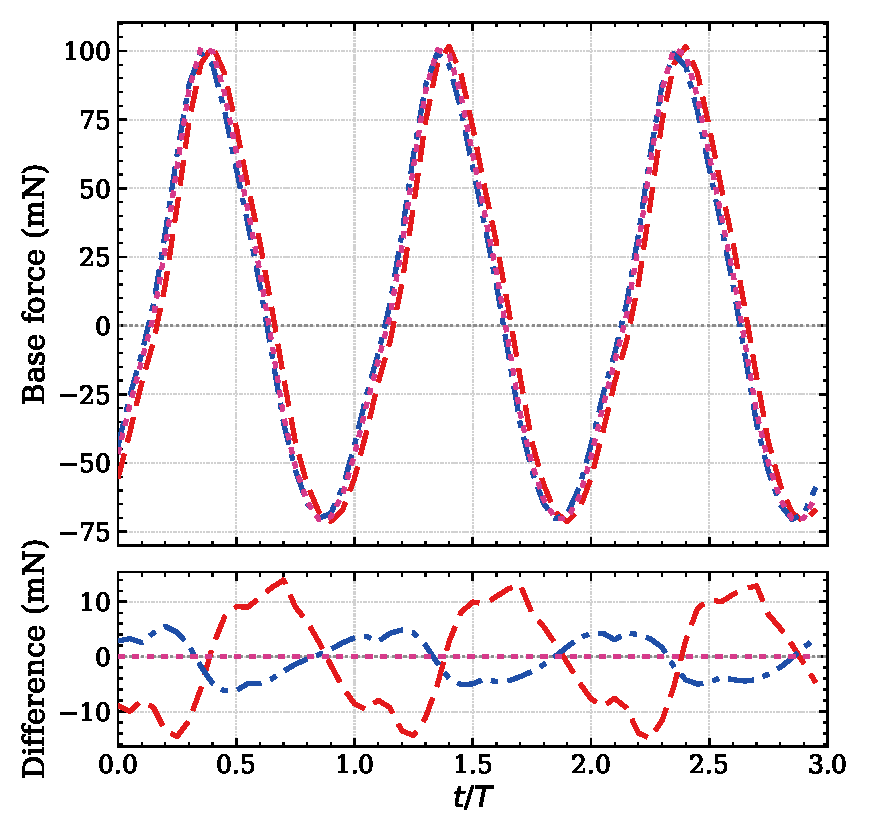
\includegraphics[width=0.70\textwidth]{mimic3_mesh_baseForce.pdf}\\[0.5em]
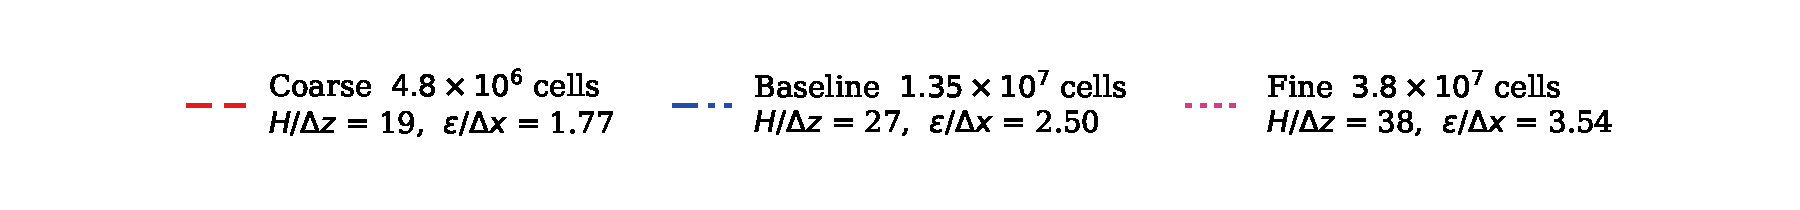
\includegraphics[width=0.95\textwidth]{mimic3_mesh_legend.pdf}
\caption{Horizontal base force on the stem over three developed wave periods at condition H110T20, on the three meshes, with the difference from the fine mesh below. The legend strip applies to this figure and to Figures~\ref{fig:flexveg_mesh_eta} and~\ref{fig:flexveg_mesh_env}. The coarse curve differs from the fine one by up to $13~\mathrm{mN}$, which is the signature of its $8.85^{\circ}$ phase lag rather than of a load-magnitude error.}
\label{fig:flexveg_mesh_force}
\end{figure}

\noindent
The free surface is where the three meshes differ most, and the difference sits almost entirely in the mean level rather than in the wave itself. The mean water level at the stem is $+1.0$, $+9.1$ and $+6.8~\mathrm{mm}$ on the three meshes, so the coarse mesh develops essentially no wave setup, and this is the least converged quantity of the study. Referenced to the still water level the coarse mesh then appears to lose $10.1\%$ of its crest, at $65.9$ against $73.3~\mathrm{mm}$, but most of that gap is the missing setup. Referenced to the local mean, which is how a wave gauge reports an elevation and how Section~\ref{sec:flexveg_results_wave} reports it, the crest runs $64.9$, $65.4$ and $66.5~\mathrm{mm}$ and the trough $-42.7$, $-44.2$ and $-44.1~\mathrm{mm}$, so the wave at the stem is reproduced to within $2.4\%$ on every mesh. The crest fraction on that datum is $0.627$, $0.624$ and $0.627$, so the crest-trough asymmetry of the Stokes wave is captured identically at all three resolutions. Figure~\ref{fig:flexveg_mesh_env} shows the same picture along the flume, the coarse envelope lying below the other two at the crest and at the trough alike, which is a shift of the mean rather than a distortion of the wave.

\begin{figure}[!ht]
\centering
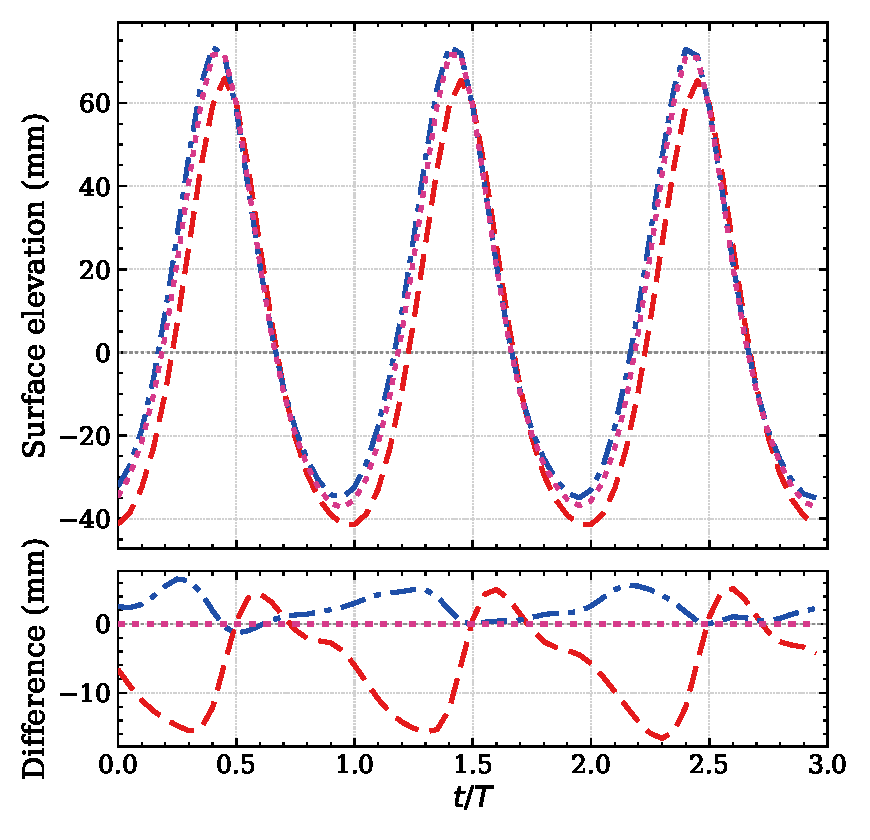
\includegraphics[width=0.70\textwidth]{mimic3_mesh_waveElevation.pdf}
\caption{Free-surface elevation at the stem over three developed wave periods on the three meshes, referenced to the still water level, with the difference from the fine mesh below. The coarse curve sits below the other two through the whole cycle, which is its missing wave setup; about the local mean the three crests agree to within $2.4\%$. Line styles follow the legend of Figure~\ref{fig:flexveg_mesh_force}.}
\label{fig:flexveg_mesh_eta}
\end{figure}

\begin{figure}[!ht]
\centering
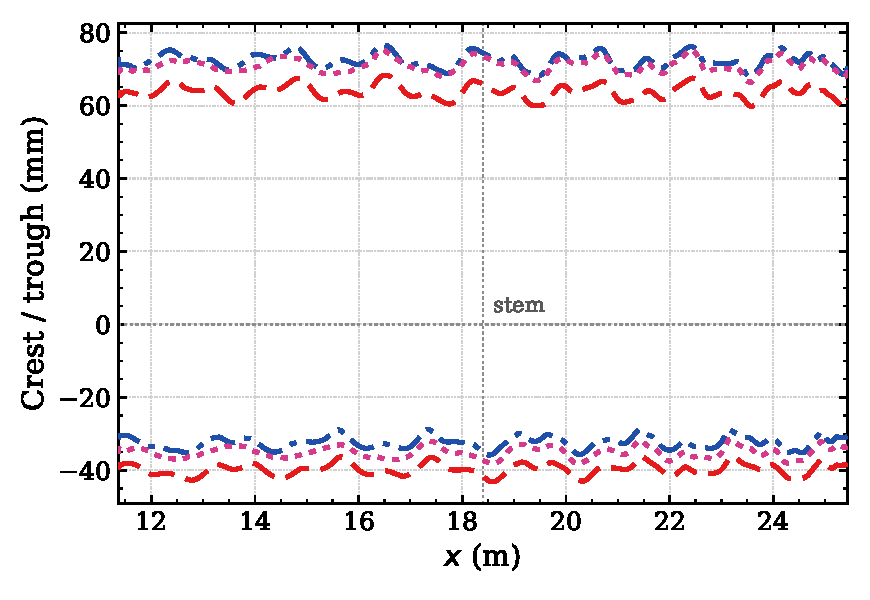
\includegraphics[width=0.70\textwidth]{mimic3_mesh_waveEnvelope.pdf}
\caption{Crest and trough envelope along the plateau on the three meshes, referenced to the still water level, with the stem location marked. The coarse envelope lies below the other two at the crest and at the trough alike, at every station rather than only at the stem, which is the signature of its missing wave setup. The $\pm5\%$ modulation along the flume is the standing-wave pattern of a weak outlet reflection. Line styles follow the legend of Figure~\ref{fig:flexveg_mesh_force}.}
\label{fig:flexveg_mesh_env}
\end{figure}

\noindent
The flume-averaged wave height converges monotonically, at $103.5$, $104.7$ and $106.0~\mathrm{mm}$ against the $110~\mathrm{mm}$ target, so all three meshes fall short of the target by $3.6$ to $5.9\%$. That deficit is not numerical damping. The local wave height is flat along the flume within a $\pm5\%$ modulation whose measured spatial period is $1.92~\mathrm{m}$ against the $1.942~\mathrm{m}$ of $\lambda/2$ from linear dispersion, which is the signature of a weak reflection off the outlet with an amplitude coefficient of about $0.05$, the same on all three meshes.

\noindent
Two limits of the study should be stated. Only three levels are available and the fine run is not fully settled, so no Richardson extrapolation was attempted. The refinement is also simultaneous in the three directions with $\varepsilon$ held fixed, so the vertical resolution of the free surface is not separated from the streamwise celerity error or from the change in $\varepsilon/\Delta x$, and an isolated vertical refinement is the run that would separate them. What the study does establish is that the load and the response, which are the quantities compared against the experiment in Section~\ref{sec:flexveg}, are insensitive to the mesh at the $2\%$ level over an eightfold change in cell count, and that the wave at the stem is reproduced to within $2.4\%$ on all three meshes once the mean level is removed. The quantity that does need the resolution is the wave setup, which the coarsest mesh fails to develop, and which enters the response only through the $1\%$ change it makes to the orbital velocity.


\end{appendices}
